\documentclass[institutional,screen,none]{../cls/ua-engineering-v6-beamer}
% !TeX encoding = UTF-8
\UASetUniversity{Universidad Austral}
\UASetFaculty{Facultad de Ingeniería}
\UASetDepartment{Departamento de Computación}
\UASetCampus{Pilar}
\UASetCareer{Ingeniería Informática}
\UASetCommission{Comisión A}
\UASetProfessor{Equipo docente}
\UASetSemester{Segundo cuatrimestre 2026}
\UASetCourse{Sistemas Distribuidos}
\UASetDate{2026}


\UASetClassNumber{05}
\UASetClassTitle{Transacciones distribuidas}

\title{\UACourse}
\subtitle{Clase 05 --- Serializabilidad, anomalías y 2PC/3PC}

\begin{document}

{
\setbeamertemplate{footline}{}
\begin{frame}[plain]
\titlepage
\end{frame}
}

\UASectionSlide{Motivación}

\begin{frame}{De orden global a correctitud}
\begin{itemize}
\item Consenso ⇒ orden total de operaciones
\item Falta: \textbf{correctitud lógica de operaciones compuestas}
\end{itemize}

\pause
\begin{block}{Problema}
¿Cómo ejecutar múltiples operaciones concurrentes sin violar invariantes?
\end{block}
\end{frame}

\begin{frame}{Transacción}
\begin{block}{Definición}
Unidad lógica de trabajo que debe ejecutarse de forma atómica y aislada.
\end{block}

\pause
ACID:
\begin{itemize}
\item Atomicidad: todo o nada
\item Consistencia: preserva invariantes
\item Aislamiento: ejecución como si fuera sola
\item Durabilidad: persistencia tras commit
\end{itemize}
\end{frame}

\UASectionSlide{Serializabilidad}

\begin{frame}{Idea central}
\begin{block}{}
Una ejecución concurrente es correcta si equivale a una ejecución secuencial.
\end{block}
\end{frame}

\begin{frame}{Grafo de precedencia}
\begin{itemize}
\item nodos: transacciones
\item aristas: dependencias por conflictos
\end{itemize}

\pause
\begin{alertblock}{Criterio}
Si el grafo tiene ciclo ⇒ no serializable
\end{alertblock}
\end{frame}

\begin{frame}{Ejemplo de ciclo}
\begin{center}
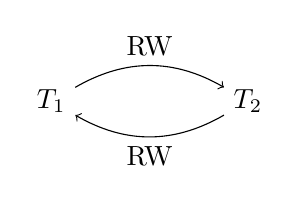
\begin{tikzpicture}[node distance=2.5cm]
\node (t1) {$T_1$};
\node (t2) [right of=t1] {$T_2$};

\draw[->] (t1) to[bend left] node[above]{RW} (t2);
\draw[->] (t2) to[bend left] node[below]{RW} (t1);
\end{tikzpicture}
\end{center}

\pause
Resultado: no existe orden secuencial equivalente
\end{frame}

\UASectionSlide{Anomalías}

\begin{frame}{Dirty read}
\begin{itemize}
\item $T_1$ escribe
\item $T_2$ lee valor no confirmado
\item $T_1$ aborta
\end{itemize}
\end{frame}

\begin{frame}{Non-repeatable read}
\begin{itemize}
\item $T_1$ lee valor
\item $T_2$ lo modifica
\item $T_1$ vuelve a leer distinto valor
\end{itemize}
\end{frame}

\begin{frame}{Phantom}
\begin{itemize}
\item $T_1$ lee conjunto
\item $T_2$ inserta nuevo registro
\item $T_1$ vuelve a leer ⇒ aparece “fantasma”
\end{itemize}
\end{frame}

\begin{frame}{Write skew}
\begin{itemize}
\item ambas transacciones leen mismo estado
\item ambas escriben sin conflicto directo
\end{itemize}

\pause
\begin{alertblock}{Clave}
Snapshot Isolation permite esto ⇒ no es serializable
\end{alertblock}
\end{frame}

\UASectionSlide{Niveles de aislamiento}

\begin{frame}{SQL estándar}
\begin{itemize}
\item Read Uncommitted
\item Read Committed
\item Repeatable Read
\item Serializable
\end{itemize}
\end{frame}

\begin{frame}{Snapshot Isolation}
\begin{itemize}
\item snapshot consistente al inicio
\item evita dirty read y non-repeatable read
\item NO evita write skew
\end{itemize}
\end{frame}

\UASectionSlide{Commit distribuido}

\begin{frame}{Problema}
\begin{block}{}
Commit en múltiples nodos debe ser atómico
\end{block}
\end{frame}

\begin{frame}{2PC}
\textbf{Fase 1: Prepare}
\begin{itemize}
\item coordinador pregunta “¿puedes committear?”
\end{itemize}

\textbf{Fase 2: Commit}
\begin{itemize}
\item si todos dicen sí ⇒ commit
\item si alguno dice no ⇒ abort
\end{itemize}
\end{frame}

\begin{frame}{Problema de 2PC}
\begin{itemize}
\item coordinador cae
\item participantes quedan bloqueados
\end{itemize}
\end{frame}

\begin{frame}{3PC}
\begin{itemize}
\item agrega fase intermedia (pre-commit)
\item reduce bloqueo
\end{itemize}

\pause
Limitación:
\begin{itemize}
\item requiere sincronía parcial
\end{itemize}
\end{frame}

\UASectionSlide{Cierre}

\begin{frame}{Idea central}
\begin{block}{}
Serializabilidad es el estándar de corrección, pero requiere coordinación fuerte.
\end{block}
\end{frame}

\end{document}
